\documentclass[two column, oneside]{article}
\usepackage[utf8]{inputenc}
\usepackage[en]{babel} %Gestor de locales

\usepackage{graphicx} %gráficos extendidos
\usepackage{float} %numeración flotante
\usepackage{fixltx2e} %subscripts
\usepackage{appendix}
\usepackage{lipsum}
\usepackage{multicol}
\usepackage{listings}

\title{ARSE Respirator}
\author{Enrique Alapont}
\date{20200409}

% Macros
\newcommand{\Vcc}{Vcc}% Vdc
\newcommand{\Vca}{Vca}% Vac


\begin{document} 
    \maketitle
    %En
    \section*{Summary}
\textit{
    This document describes the first design for a simple emergency respirator. Its simplicity will ease understanding, manufacture, use, maintenance and recycling.
}\\
\\
\textbf{Key words:} respirator, ventilator
    \section{Introduction}
\subsection{Target}
    Due to the actual health crisis ¡ (2020 march) and troublesome forecasts, is interesting to have an easy to manufacture respirator, made with widely available elements, which will help breathing to sick people with the coronavirus COVID-19 without excessive external requirements.\\
    
    A plug should be enough to work, without the need of pressure air or other requirements, although it is possible to add oxygen enriched air to the entrance.
    
\subsection{Requirements}
    The respirator will be "not invasive", will contribute with pressure air to the patient via a face mask. Breathing timing are adjustable both in duration and strength. Exhale cycles are passive, with positive pressure and adjustable in duration.\\
    
    Specifications have been chosen to the effect published at the United Kingdom \cite{MHRA} due to its completeness and realisticness, on the current circumstances.\\
    
    It needs to be cheap and fast to build, have an easy and comprehensible use, and use cheap and widely available components. It is built with non polluting material, nor in its operation nor in its disposal.\\
    
    It will also comply with requirements imposed by the Agencia Española de Medicamentos y Productos Sanitarios (Spanish Drug and Sanitary Products)
    
    \section{Design}
\subsection{Overview}
    \begin{figure}[H]
        \centering
        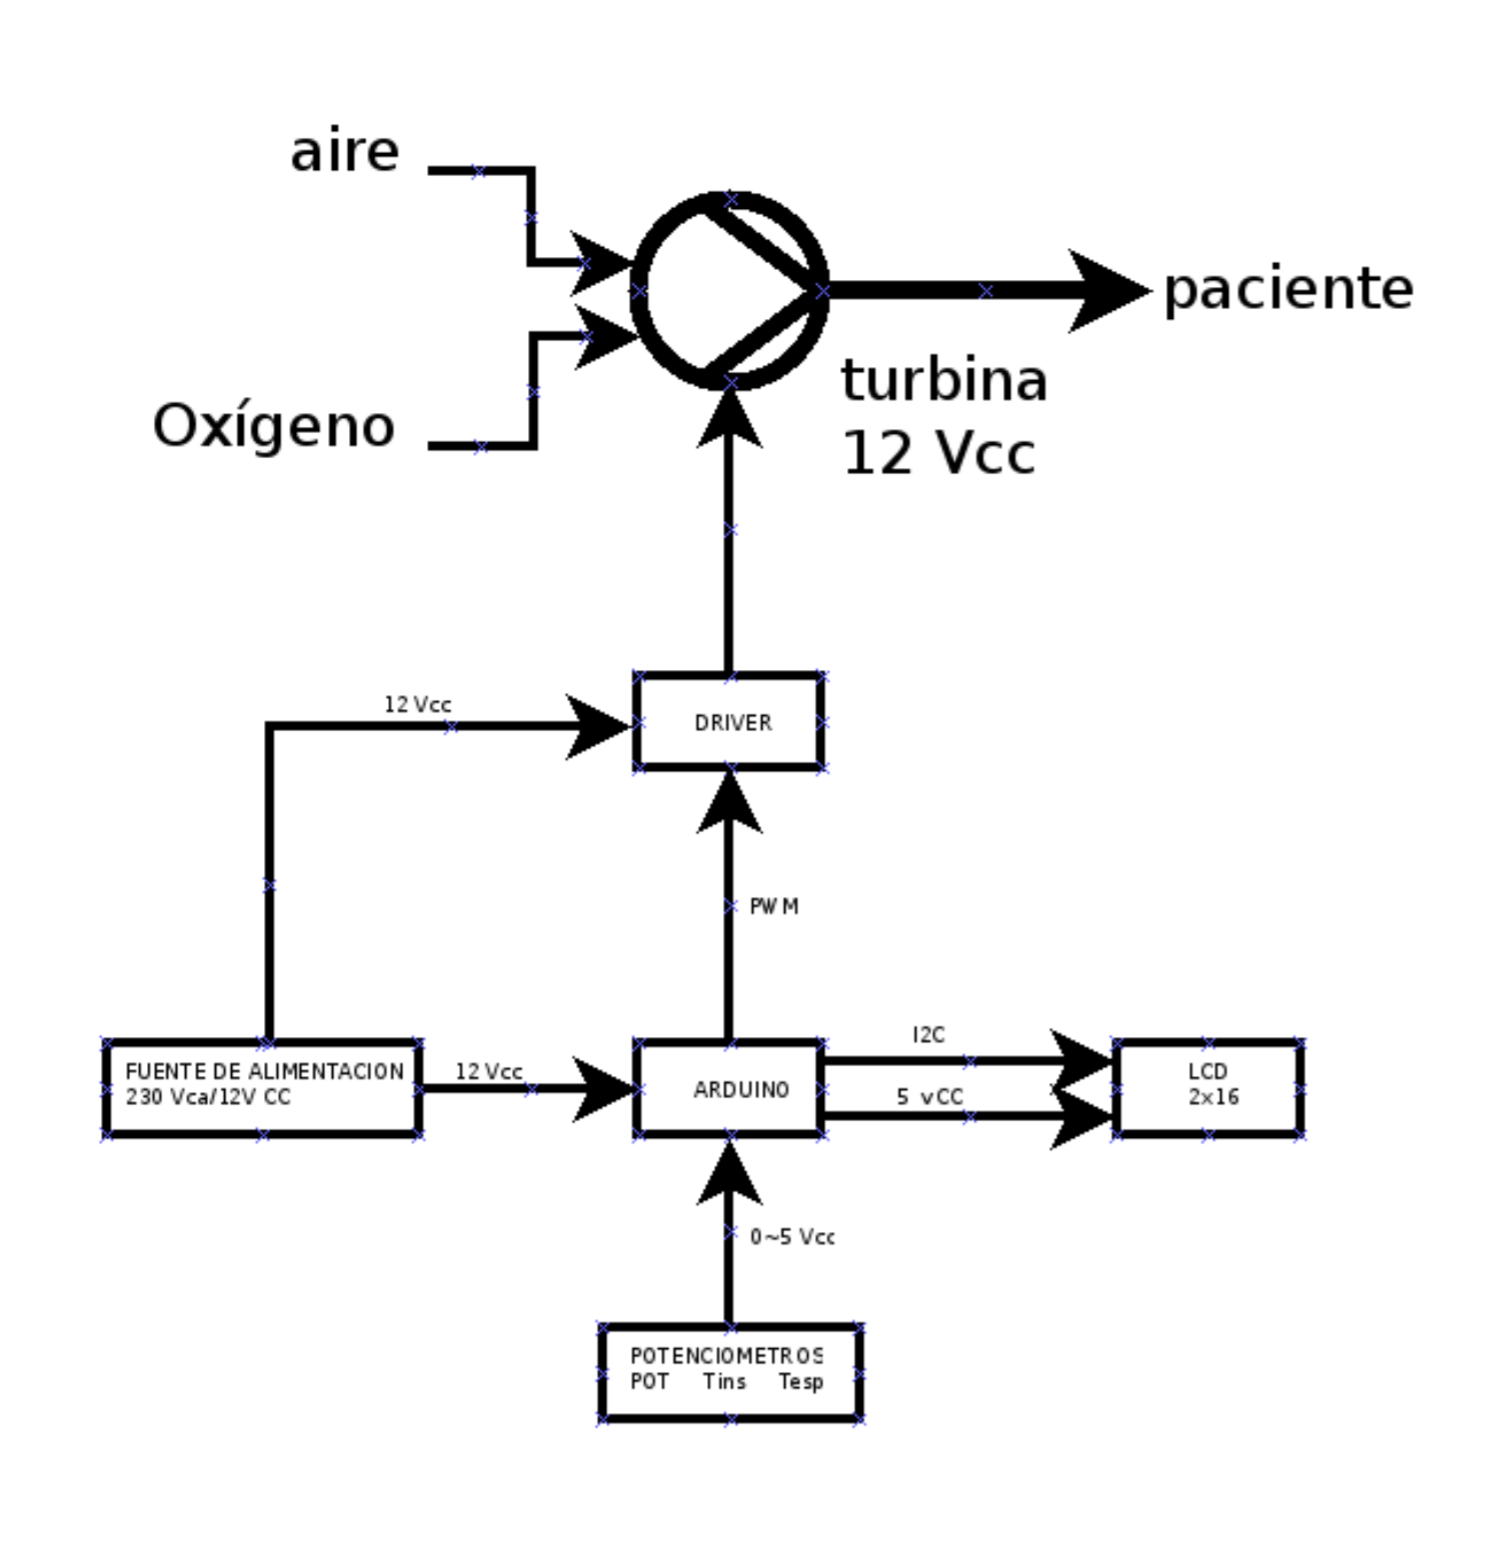
\includegraphics[width=0.4\textwidth]{Img/Bloques.PNG}
        \caption{Block diagram}
    \end{figure}
    The respirator is composed of an air turbine, an electronic board, a power supply and a plastic case.\\
    
    The driving turbine collects air (medical or atmospheric) and oxygen and will drive it to the patient at the rhythm and pressure determined by medical staff. This turbine will be powered from an electronic board, which contains the control system (microcontroller) and a display. The controlling elements are three potentiometers located on the front panel (transparent) and connected to the board by wires. A power 12 \Vcc supplies power to the electronics, and via the electronics, the turbine. The device can be powered by an ambulance battery at 12 \Vcc. The plastic case with a transparent front panel, makes the electrical enclosure isolating the device.
    
    %La turbina impulsora recoge aire (medicinal o atmosférico) y Oxígeno y lo lleva hasta el paciente con el ritmo y presión que determine el personal sanitario. Esa turbina está alimentada desde una placa electrónica que contiene el sistema de control (microcontrolador) y la pantalla. Los elementos de mando son tres potenciómetros situados en la tapa frontal (transparente) y conectados a la placa electrónica por cables. Una fuente de 12 \Vcc alimenta a la electrónica y a través de esta, a la turbina. El equipo puede ser alimentado por la batería de 12 \Vcc de una ambulancia. Por último, una caja de plástico con el frontal transparente constituye la envolvente eléctrica que dota de aislamiento al conjunto.
    
    All the maneuver, parameters and limit values are defined by software.
    %Toda la maniobra y los valores de los parámetros y los valores límite de las variables están definidos por software.
    \begin{figure}
        \centering
        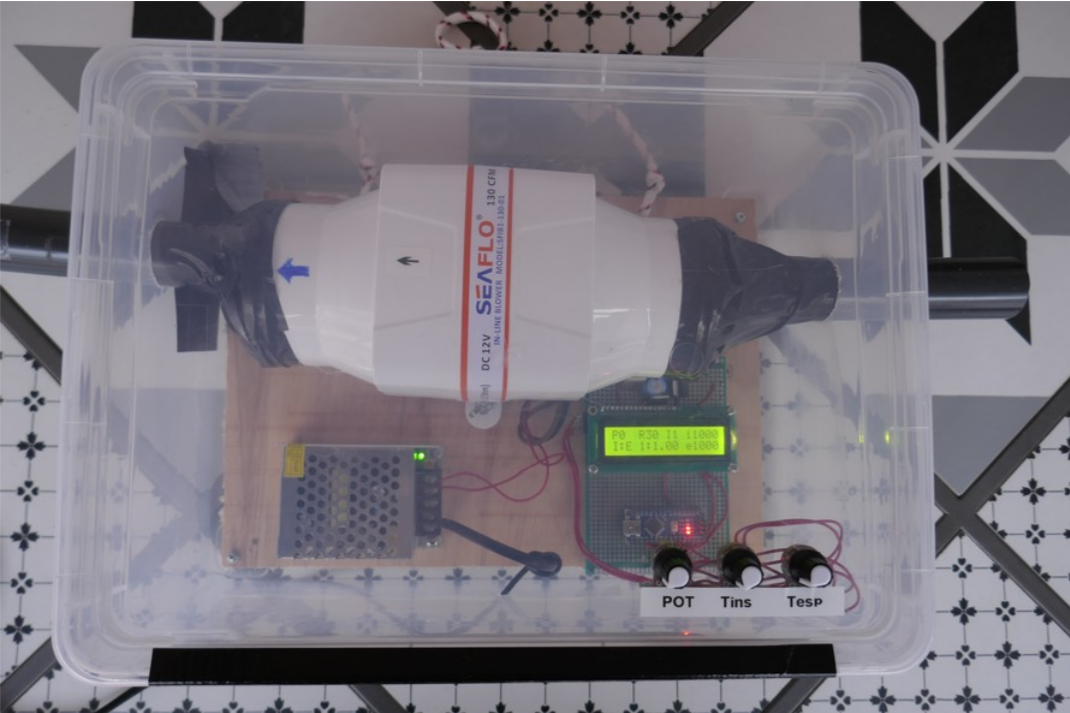
\includegraphics[width=0.4\textwidth]{Img/prototipo-1.PNG}
        \caption{First prototype}
    \end{figure}
    
\subsection{Turbine}
    The electric motor blower at 12\Vcc or 24\Vcc is controlled by a pulse width modulated power transistor. The one used in the prototype comes from the nautic market (it is a bilge ventilator)\\    
    %El soplador con motor eléctrico de 12 \Vcc o de 24 \Vcc está controlado por un transistor de potencia con modulación por anchura de pulso. El usado en el prototipo procede del mercado náutico (es un ventilador de sentina).\\
    It must be able to blow 600ml (excepcionally 800ml) at a preassure up to 70cmH\textsubscript{2}O
    %Debe ser capaz de soplar 600 ml (800 ml excepcionalmente) a una presión de hasta 70 cmH\textsubscript{2}0\\
    If an alternating current blower was needed, would force to redesign both the hardware and the software (can be done fast).
    %Si hiciera falta usar un ventilador de corriente alterna a 230\Vca, debería rediseñarse tanto el hardware como el software (puede hacerse muy rápidamente).

\subsection{Electronic Board}
    The electronic board incorporates the following elements:
    %La tarjeta electrónica incorpora los siguientes elementos:
    \begin{itemize}
        \item Current stabilizer  %Estabilizador de tensión
        \item Display %Pantalla
        \item Computer %Ordenador
        \item Motor signal amplifyer  %Amplificador de salida al motor
    \end{itemize}
    The current stabilizer objective is to supply at 5 \Vcc all the electronic active components. It is composed by an integrated regulator type \textit{7805} in a box \textit{TO220} without radiator, with filtered capacitors an input and output.\\
    %   El estabilizador de tensión tiene por objeto alimentar a 5 \Vcc a todos los elementos electrónicos activos. Está compuesto por un regulador integrado tipo \textit{7805} en caja \textit{TO220} sin radiador, con condensadores de filtro en la entrada y en la salida.\\

    The display is a retro iluminated, two lines, 16 character display. It is connected to the computer via an \textit{I2C} serial bus.\\
    %La pantalla es del tipo LCD retroiluminada de dos filas de 16 caracteres, conectada al ordenador mediante un bus serie tipo \textit{I2C}.\\
    
    The computer is an \textit{Arduino Nano} build with a micro controller ATMEL \textit{ATmega328}. The program is design in the \textit{Arduino} environment and loads in the computer flash memory via USB interface. It is easy and cheap to obtain at around 3€.\\
    %El ordenador es un modelo \textit{Arduino Nano} construido desde un microcontrolador ATMTEL \textit{ATmega328}. El     programa está desarrollado en el entorno \textit{Arduino} y se carga en memoria flash del ordenador por el interface USB. Se puede conseguir fácilmente en el mercado y es muy barato (desde 3€).\\
    
    The motor output amplifier is built by a middle power NPN Darlington transistor type \textit{TIP120}. It is design to be able to use FET-MOS transistos, encapsulated with the case design (TO220), like the \textit{IRF3710}.\\
    %El amplificador de salida del motor está constituido por un transistor de media potencia NPN en montaje Darlington tipo \textit{TIP120} y está diseñado para poder usar transistores FET-MOS encapsulados en el mismo tipo de caja (TO220), como el \textit{IRF3710}.
    
\subsection{Potentiometers}
    The control elements consist of three linear potentiometers mounted over a printed circuit board. These control maximum power, inhaling time and exhale time. The three are mounted over the front pannel to make them accessible.\\
    %Tres potenciómetros lineales montados sobre un pequeño circuito impreso constituyen los elementos de control sobre potencia máxima de la turbina, tiempo de inspiración y tiempo de espiración. Los tres están montados sobre la tapa frontal para hacerlos accesibles.\\
    
    Limit values, both minimum and maximum for each potentimeter are software defined, as the magnitudes controlled by each one. Making modifications easy.
    %Los valores límite máximo y mínimo de cada potenciómetro están definidos por software, así como las propias magnitudes que controlan, con lo que pueden modificarse fácilmente.

\subsection{Case}
    The set is mounted over a mounting plate, screwed over the bottom of the case. This must provide both structural sturdiness and mechanical and electrical shielding needed in a medical enviroment. It must be posible to be cleaned and disinfected while working.\\ 
    %Todo el conjunto se monta sobre una placa de montaje que a su vez se atornilla sobre el fondo de la caja. Esta debe proveer, no solo la robustez estructural del conjunto, sino también la protección mecánica y eléctrica necesaria en un entorno hospitalario. De ser capaz de ser limpiada y desinfectada en funcionamiento.\\
    
    Final working products will be comercial plastic enclosures with the propper characteristics and a transparent pannel.
    %Los ejemplares de producción final serán envolventes plásticas comerciales de las característica adecuadas con tapa transparente.
    \section{Build}
    The electronic circuits are mounted over a printed circuit board. The display is  mounted with spacers over the circuit and connected with a flat 8 wire cable. The Arduino is mounted over the socket, everything else is soldered. Everything is mounted at the mounting plate, except the electronic circuit, whitch uses 5mm spacers.\\
    %Los circuitos electrónicos se montan sobre circuito impreso. El display se monta con separadores sobre el circuito y va conectado con un cable plano de 8 hilos. El Arduino va sobre zócalo, lo demás, soldado. Todo sobre la placa de montaje directamente, excepto el circuito electrónico, que va sobre separadores de 5 mm.\\
    The back plate is mounted with the case screws, the turbine uses M4 pins, everything else will use M3 screws. 
    %La placa trasera se monta con la tornillería que lleve la caja, La turbina, com pernos M4, todo lo demás con tornillería M3.
    \section{Operation}
    Turbine power will be selected from the front panel (0 to 100\%), inhaling and exhaling time (with minimum and maximums software defined).\\
    %Desde el panel frontal se seleccionará la potencia de la turbina (de 0 a 100\%), el tiempo de inspiración (desde mínimo a máximos programados) y el tiempo de espiración (con mínimo y máximo programados).\\
    
    The display provides the following information:
    %El display ofrece la siguiente información:
    \begin{itemize}
        \item Top row
        \begin{itemize}
            \item[--] P: Power, from 0 to 99\%
            \item[--] R: Breaths per minute (BPM) \footnote{Translator's Note: Respiraciones Por Minuto in original Spanish, therefore the R}
            \item[--] E/I Actual phase: I0, I1, E0, E1
            \item[--] i: Inhaling time, secconds
        \end{itemize}
        \item Bottom row
        \begin{itemize}
            \item[--] I:E: Inhale/Exhale ratio
            \item[--] E: Exhaling time
        \end{itemize}
    \end{itemize}
    
    The routine completes the inhale-exhale cycle in four phases: I0, I1, E0 and E1. Phases I0 and E0 are brief and only used for technical adjustements (E.g. the motor start). Almost the whole Inhaling is done at I1. E0 is not used.
    %El programa lleva a cabo el ciclo inspiración+espiración en cuatro fases: I0, I1, E0 y E1 en las que las fases I0 y E0 son muy breves y solo se usan para ajustes técnicos (como la arrancada del motor, por ejemplo), la casi totalidad de la inspiración se lleva a cabo en I1. E0 no se usa actualmente\\
    
    The selected times corresponds to:
    %Los tiempos seleccionados corresponden a;
    \begin{itemize}
        \item Inhale time: I0 + I1
        \item Exhale time: E0 + E1
    \end{itemize}
    
    In the actual design, the timing ratio is produced by selecting inhaling and exhaling time, showing Breaths Per Minute \footnote{TN: RPM in the original and R: in the screen} and its ratio I:E. It can be easily changed in the software for the potentiometers to select I:E ratio and Breaths Per Minute.
    %En el actual diseño la selección de tiempos se hace escogiendo los tiempos de inspiración y espiración y mostrando las RPM y la relación I:E. Puede fácilmente cambiarse el programa para que los potenciómetros seleccionen la relación I:E y las RPM.
    \section{Maintenance}
    Inside maintenance is nil. Externally, the respirator must be sponge washed and disinfected when aplicable.
    %El mantenimiento necesario en el interior es nulo. Externamente el respirador deberá ser lavado con una esponja y desinfectado cuando proceda. 
    \section{Destruction and Recycling}
    The device is conceived to work full time for a few months. At the end of the exceptional situation, which has motivated its design, it must be destroyed. It must be considered as bio-contaminated and must be disposed accordingly.
    %El aparato está concebido para funcionar contínuamente  unos pocos meses. Al terminar la situación de excepcionalidad que ha motivado su construcción, será destruido. Deberá ser considerado como biocontaminado y procederse en consecuencia.

    %Es
    %\section*{Resumen}
\textit{
    El presente documento describe un primer diseño de un respirador sencillo para situaciones de emergencia. Su simplicidad facilitará la comprensión, la fabricación, el uso, el mantenimiento y el reciclado.
}\\
\\
\textbf{Palabras Clave:} respirador, ventilador
    %\section{Introducción}
\subsection{Objetivo}
    Dada la actual situación sanitaria (marzo de 2020) y las preocupantes previsiones de futuro, interesa disponer de un modelo de respirador que permita su fabricación masiva con elementos fácilmente disponibles en el mercado y que permita ayudar a respirar a personas afectadas por el coronavirus COVID-19 sin excesivos requerimientos externos. Un enchufe debe ser suficiente para que funcione, sin necesitar de aire a presión ni otros requerimientos, aunque es posible el aporte de aire enriquecido con oxígeno en la toma de entrada.
\subsection{Requisitos}
    El respirador será “no invasivo”, aportará aire a presión al paciente por medio de una mascarilla. Los tiempos de inspiración serán regulables en duración e intensidad. Los ciclos de espiración serán pasivos, con presión positiva y regulables en duración.\\
    Se han escogido las especificaciones al efecto publicadas en el Reino Unido \cite{MHRA} por ser bastante completas y realistas, dadas las circunstancias.\\
    Deberá ser barato y rápido de construir, con funcionamiento sencillo y comprensible y componentes  económicos y fáciles de conseguir. Se emplearán materiales no contaminantes, ni en su operación ni en su destrucción.\\
    También deberá cumplir con los requisitos que exige la Agencia Española de Medicamentos y Productos
    Sanitarios. 
    %\section{Diseño}
\subsection{Visión de conjunto}
    \begin{figure}[H]
        \centering
        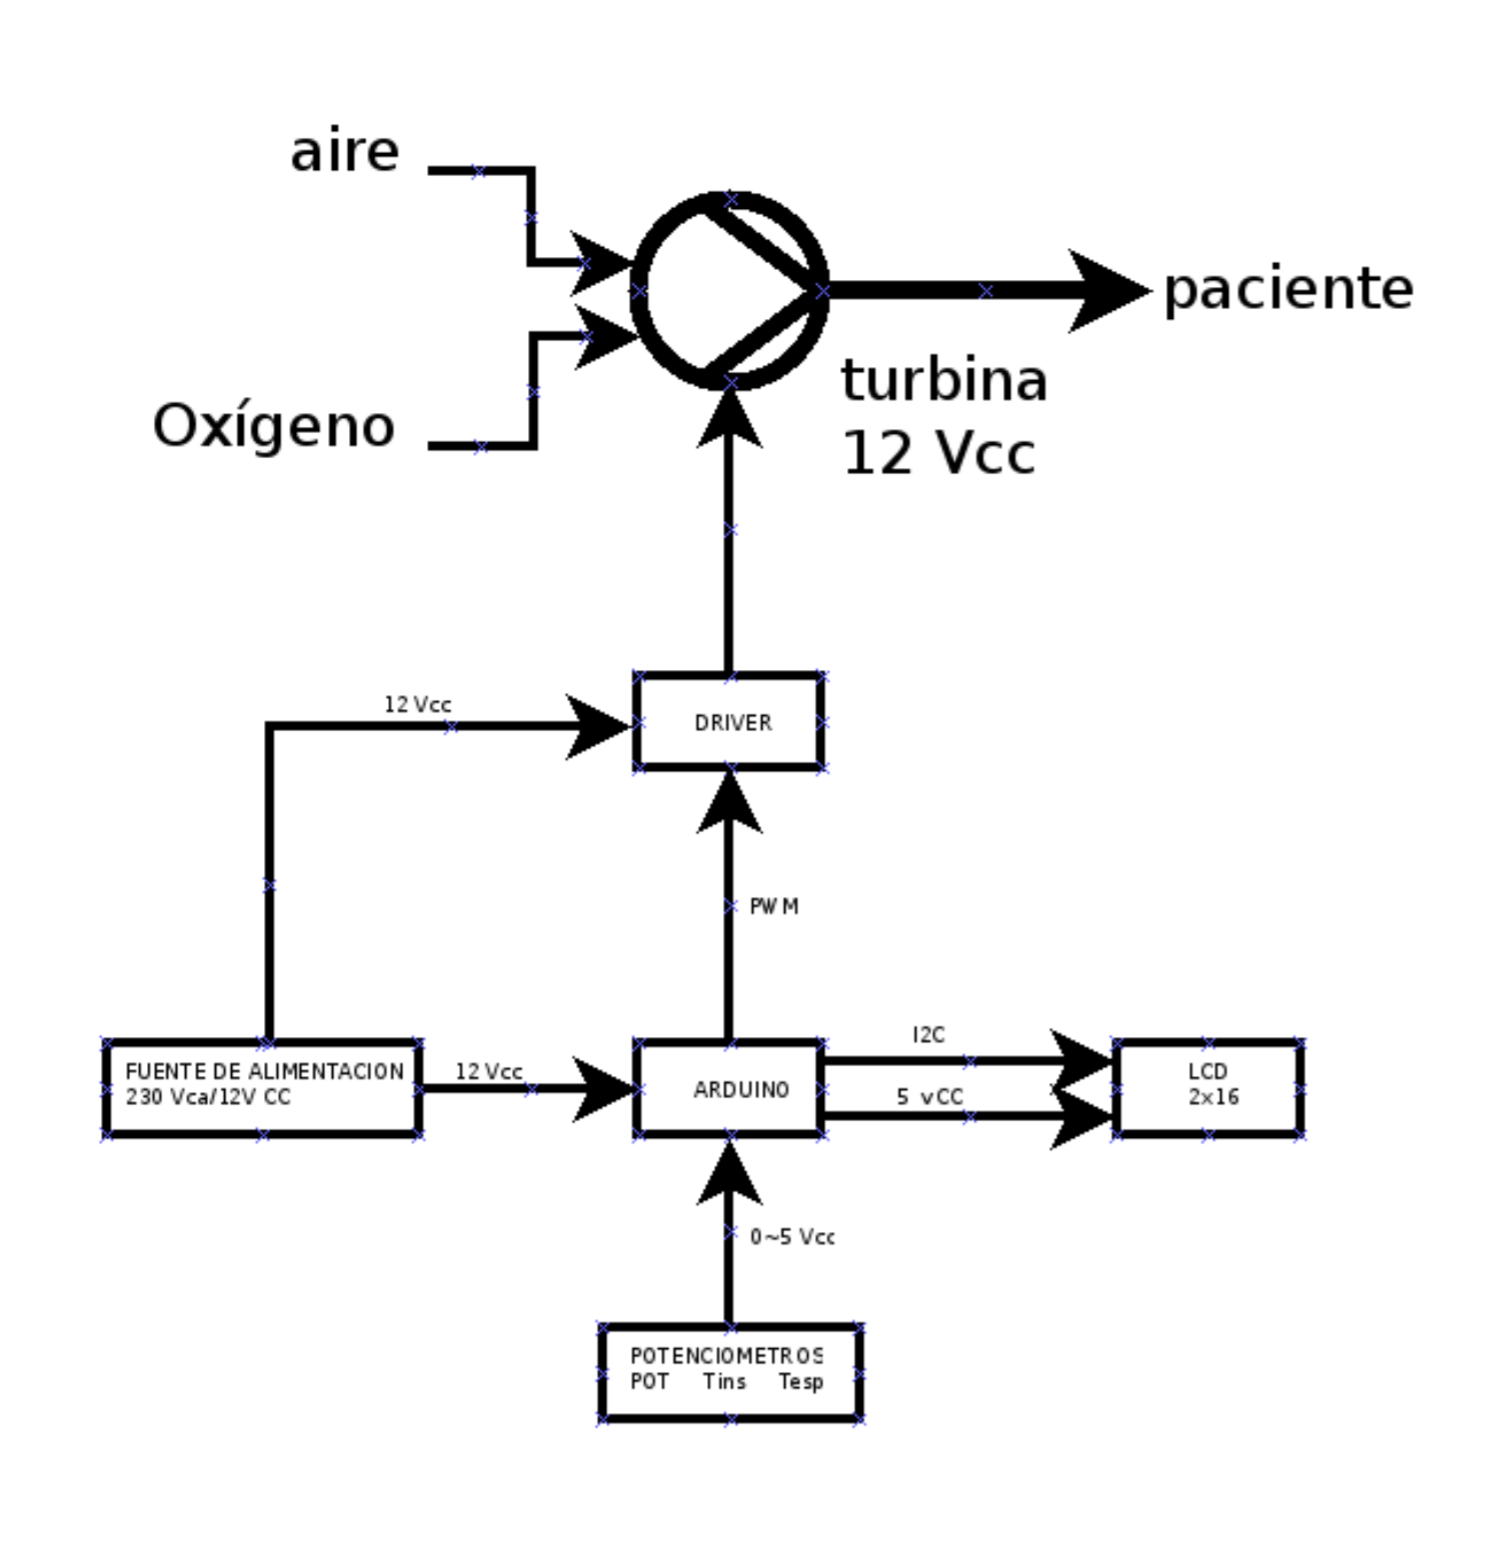
\includegraphics[width=0.4\textwidth]{Img/Bloques.PNG}
        \caption{Esquema de bloques}
    \end{figure}
    El respirador está compuesto por una turbina de aire, una tarjeta electrónica una fuente de alimentación y una caja de plástico.\\
    
    La turbina impulsora recoge aire (medicinal o atmosférico) y Oxígeno y lo lleva hasta el paciente con el ritmo y presión que determine el personal sanitario. Esa turbina está alimentada desde una placa electrónica que contiene el sistema de control (microcontrolador) y la pantalla. Los elementos de mando son tres potenciómetros situados en la tapa frontal (transparente) y conectados a la placa electrónica por cables. Una fuente de 12 \Vcc alimenta a la electrónica y a través de esta, a la turbina. El equipo puede ser alimentado por la batería de 12 \Vcc de una ambulancia. Por último, una caja de plástico con el frontal transparente constituye la envolvente eléctrica que dota de aislamiento al conjunto.
    
    Toda la maniobra y los valores de los parámetros y los valores límite de las variables están definidos por software.
    \begin{figure}
        \centering
        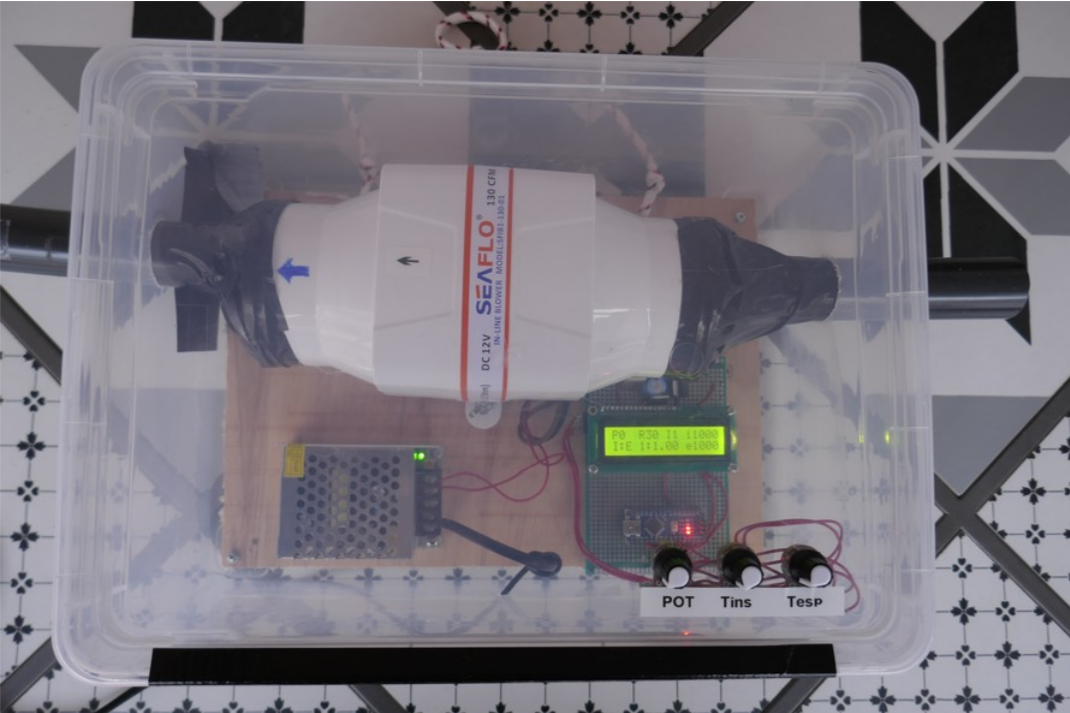
\includegraphics[width=0.4\textwidth]{Img/prototipo-1.PNG}
        \caption{Primer prototipo}
    \end{figure}
    
\subsection{Turbina}
    El soplador con motor eléctrico de 12 \Vcc o de 24 \Vcc está controlado por un transistor de potencia con modulación por anchura de pulso. El usado en el prototipo procede del mercado náutico (es un ventilador de sentina).\\
    Debe ser capaz de soplar 600 ml (800 ml excepcionalmente) a una presión de hasta 70 cmH\textsubscript{2}0\\
    Si hiciera falta usar un ventilador de corriente alterna a 230\Vca, debería rediseñarse tanto el hardware como el software (puede hacerse muy rápidamente).
\subsection{Tarjeta Electrónica}
    La tarjeta electrónica incorpora los siguientes elementos:
    \begin{itemize}
        \item Estabilizador de tensión
        \item Pantalla
        \item Ordenador
        \item Amplificador de salida al motor
    \end{itemize}
    El estabilizador de tensión tiene por objeto alimentar a 5 \Vcc a todos los elementos electrónicos activos. Está compuesto por un regulador integrado tipo \textit{7805} en caja \textit{TO220} sin radiador, con condensadores de filtro en la entrada y en la salida.\\

    La pantalla es del tipo LCD retroiluminada de dos filas de 16 caracteres, conectada al ordenador mediante un bus serie tipo \textit{I2C}.\\
    
    El ordenador es un modelo \textit{Arduino Nano} construido desde un microcontrolador ATMTEL \textit{ATmega328}. El     programa está desarrollado en el entorno \textit{Arduino} y se carga en memoria flash del ordenador por el interface USB. Se puede conseguir fácilmente en el mercado y es muy barato (desde 3€).\\
    
    El amplificador de salida del motor está constituido por un transistor de media potencia NPN en montaje Darlington tipo \textit{TIP120} y está diseñado para poder usar transistores FET-MOS encapsulados en el mismo tipo de caja (TO220), como el \textit{IRF3710}.
    
\subsection{Potenciómetros}
    Tres potenciómetros lineales montados sobre un pequeño circuito impreso constituyen los elementos de control sobre potencia máxima de la turbina, tiempo de inspiración y tiempo de espiración. Los tres están montados sobre la tapa frontal para hacerlos accesibles.\\
    Los valores límite máximo y mínimo de cada potenciómetro están definidos por software, así como las propias magnitudes que controlan, con lo que pueden modificarse fácilmente.
\subsection{Fuente de alimentación}
    La fuente de alimentación es un modelo disponible en todos los comercios especializados. Las características de tensión e intensidad vienen dadas por los requerimientos de la turbina, 12Vcc/2.5A. Por eso la fuente escogida es de 12Vcc/5A.
\subsection{Caja}
    Todo el conjunto se monta sobre una placa de montaje que a su vez se atornilla sobre el fondo de la caja. Esta debe proveer, no solo la robustez estructural del conjunto, sino también la protección mecánica y eléctrica necesaria en un entorno hospitalario. De ser capaz de ser limpiada y desinfectada en funcionamiento.\\
    Los ejemplares de producción final serán envolventes plásticas comerciales de las característica adecuadas con tapa transparente.
    %\input{Sections/Construcción}
    %\input{Sections/Operación}
    %\section{Mantenimiento}
    El mantenimiento necesario en el interior es nulo. Externamente el respirador deberá ser lavado con una esponja y desinfectado cuando proceda. 
    \input{Sections/Destrucción}
    
    %Auto
    \clearpage
    \listoffigures
    \bibliographystyle{unsrt}
    \bibliography{biblio}
    
    %appendix
    \onecolumn
    \appendix
    \appendixpage
    \section{Programa}
\lstinputlisting[language=C]{respirador.c}
    
\end{document}
